\chapter{On Formal Languages}

Hopcroft, Motwani and Ullman define a language $\mathcal{L}$ as a set of strings chosen from $\Sigma^*$, where $\Sigma$ is a particular alphabet. $\Sigma^*$ denotes the \emph{universal language}, which is the language formed by all possible sequences over an alphabet $\Sigma$. An alphabet is defined as a finite, nonempty set of symbols. \cite{hopcroft-automata}

Furthermore, they define a string or word as a finite sequence of symbols chosen from an alphabet $\Sigma$. Therefore, a word can also be seen as a concatenation of symbols that start with the \emph{empty} or \emph{identity} symbol, $\epsilon$.

However, not every word formed by the alphabet necessarily belongs to a language, since for each language, a specific set of rules exist that define \emph{membership} - whether a word belongs to the language or not.

Furthermore, it is important to note the existence of the \emph{empty language}, $\varnothing$, that is, the language that does not contain any words, not even the empty one - $\epsilon \notin \varnothing$.

The only constraint on what can be a language is that, by definition, alphabets are finite, therefore, even though there might be an infinite amount of strings in a language, they all stem from a finite alphabet \cite{hopcroft-automata}.

Chomsky defines a grammar as a ``device that enumerates the sentences of a language'' and proposes a set of restrictions that limit these grammars to different types of automata, in a way that the ``languages that can be generated by grammars meeting a given restriction constitute a proper subset of those that can be generated by grammars meeting the preceding restriction" \cite{chomsky-hierarchy}. 

Furthermore, Chomsky proposes that these grammars, ordered by increasing restrictions, can be recognized by different automata - Turing machines, linear-bounded automata (LBA), pushdown automata (PDA) or Finite State Machines (FSM), as seen in \ref{fig:chomsky-fig}.

For this work, we will focus on Type-2, or Context-Free Grammars, which can be recognized by pushdown automata, which have a ``natural, recursive notation'' \cite{hopcroft-automata}. For example, palindromes are a context-free language, as the grammar that generates it is also context-free.

\begin{figure}[h]
    \centering
    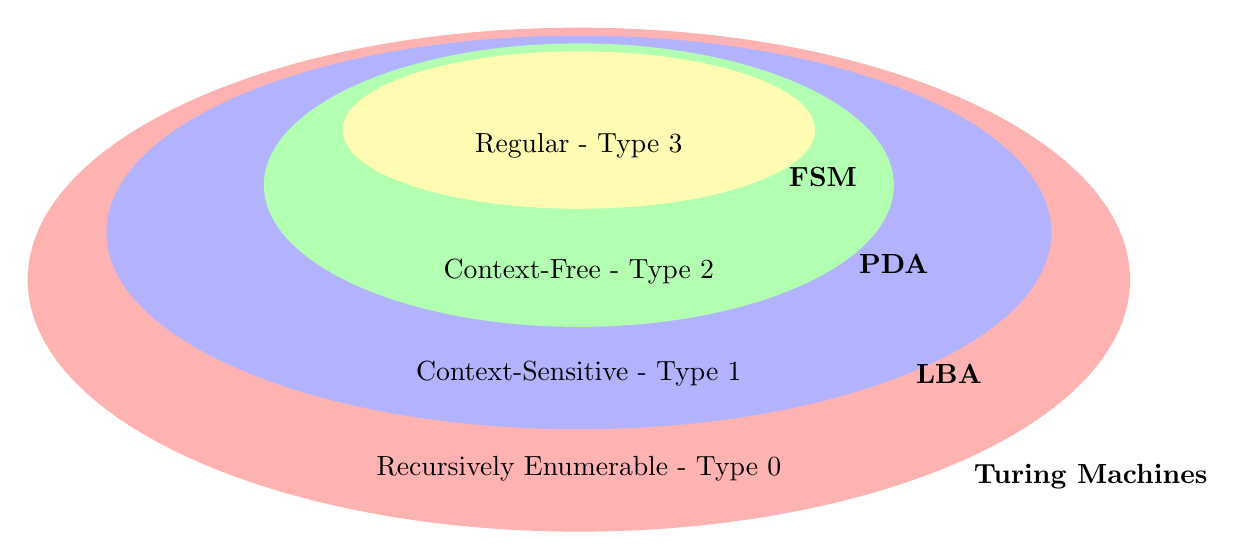
\begin{tikzpicture}
        % Draw ellipses for each language class
        \fill[red!30] (0, -0.2) ellipse (7 and 3.2);
        \fill[blue!30] (0, 0.4) ellipse (6 and 2.5);
        \fill[green!30] (0, 1) ellipse (4 and 1.8);
        \fill[yellow!30] (0, 1.7) ellipse (3 and 1);
    
        % Add labels inside each ellipse
        \node at (0, -2.6) {Recursively Enumerable - Type 0};
        \node at (0, -1.4) {Context-Sensitive - Type 1};
        \node at (0, -0.1) {Context-Free - Type 2};
        \node at (0, 1.5) {Regular - Type 3};

        \node at (3.1, 1.1) {\textbf{FSM}};
        \node at (4, 0) {\textbf{PDA}};
        \node at (4.7, -1.4) {\textbf{LBA}};
        \node at (6.5, -2.7) {\textbf{Turing Machines}};
    
    \end{tikzpicture}
    \caption{Chomsky Hierarchy}
    \label{fig:chomsky-fig}
\end{figure}

\section{Context-Free Grammars}

A context free grammar $\mathcal{G}$ has four main components \cite{hopcroft-automata}\cite{leeuwen-cfg}:
\begin{enumerate}
    \item A finite set of \emph{variables} $\mathbf{V}$ - these variables represent a language (a set of strings). We note $\mathbf{V}^*$ as the Kleene closure of the set of variables - in essence, the concatenation of zero or more repetitions of elements in the set.
    \item A finite set of symbols $\mathbf{T}$, called \emph{terminals}. Note that $\mathbf{T} \subset \mathbf{V}$. Once again, $\mathbf{T}^*$ is the Kleene closure of the set.
    \item A \emph{start symbol} $\mathbf{S} \in \mathbf{V}-\mathbf{T}$.
    \item A finite set of \emph{productions}, $\mathbf{P} \subset (\mathbf{V}-\mathbf{T})\times \mathbf{V}^*$. These represent the recursive definition of the language. Each production consists of the following:
    \begin{enumerate}
        \item A variable, called the \emph{head} that is partially defined by the production.
        \item A production symbol $\rightarrow$
        \item A string of zero or more terminals and variables, called the \emph{body}.
    \end{enumerate}
\end{enumerate}

Therefore, a grammar $\mathcal{G}$ can be expressed as a four-tuple $(\mathbf{V}, \mathbf{T}, \mathbf{P}, \mathbf{S})$. 

Given 2 words, $u, v \in \mathbf{V}^*$, we say that $u \rightarrow v$ if there exists a derivation, or sequence of words in $\mathbf{V}^*$ such that $u_{i-1} \rightarrow u_{i}$ for $i = 1,\dots,k$ and $u_0=u$ and $v=u_k$. The existence of a derivation is noted by $u \xrightarrow{*} v$

Furthermore, we define the \emph{language $\mathcal{L}$ generated by $\mathcal{G}$} as the following set:
$$
\mathcal{L}(\mathcal{G}) = \{w \in \mathbf{T}^* | \mathbf{S} \xrightarrow{*} w \}
$$
Should $X$ be a variable in $\mathcal{G}$, then:
$$
\mathcal{L}_{\mathcal{G}}(X) = \{ w \in \mathbf{T}^* | X \xrightarrow{*} w\}
$$
From this, we derive that $\mathcal{L}(\mathcal{G}) = \mathcal{L}_{\mathcal{G}}(S)$

\section{Dyck-$k$ Languages}